\subsection{Home Page}
L'Home Page è come la vetrina di un negozio: deve presentare in modo veloce, essenziale ed efficace ciò che il sito offre, e deve essere in grado in tempi molto veloci di offrire agli utenti una panoramica generale del sito e convincerli a rimanere. 
Per raggiungere in modo efficace ciò è necessario offrire informazioni relativi ai sei assi informativi che verranno trattati nella sezione \ref{6w}.\\
 \\
Le seguenti foto rappresentano la Home Page del sito raggiungibile al link \url{itstecnologie.com}. Gli screenshot qui presenti risalgono al 21 giugno 2018.
\IMG{"Home Page - Scroll 1"}
\IMG{"Home Page - Scroll 2"}
\IMG{"Home Page - Scroll 3"}
\IMG{"Home Page - Scroll 4"}
\IMG{"Home Page - Scroll 5"}
\IMG{"Home Page - Scroll 6"}
\IMG{"Home Page - Scroll 7"}
\IMG{"Home Page - Scroll 8"}

\subsubsection{I Sei Assi Informativi}\label{6w}

\paragraph{Where - In che sito sono arrivato?}
Come mostra la figura \ref{"Home Page - Scroll 1"}, quando l'utente arriva all'Home Page incontra il logo "ITS" in alto a sinistra, un menu e una grande immagine con un apparente pulsante riportante la scritta "INNOVAZIONE". \\
L'asse non viene qui soddisfatto: non c'è nessuna informazione sul sito, su cosa offre o cosa fa. La grande immagine che occupa tutta la prima vista è inutile e priva di contenuto. L'unico elemento testuale è lo slogan "Esperienza e Innovazione", privo di significato concreto anch'esso. \\
Sotto tale slogan, in grigio molto chiaro, con un contrasto quasi nullo con lo sfondo bianco, indica che la Home Page continua. Il non rendere più evidente questa cosa può essere un elemento di disorientamento per l'utente, che potrebbe essere tentato di abbandonare il sito a causa di mancanza di informazione.\\ \\
Al secondo scroll, mostrato in figura \ref{"Home Page - Scroll 2"}, si trova del testo che offre una risposta a questo asse, anche se poco chiara e troppo "romanzata". Le dimensioni del testo e l'assenza di ancore visive (come parole chiave in grassetto) rendono comunque difficoltosa la lettura. \\
\\
Procedendo con gli scroll troviamo delle presentazioni di prodotti e altre informazioni che permettono di comprendere meglio il settore in cui opera questa azienda.
\paragraph{Who - Chi rappresenta il sito?}
Il logo in alto a sinistra rappresenta il nome dell'azienda, ma tale informazione non è ben chiara se non si legge il testo visibile allo scroll 2 (figura \ref{"Home Page - Scroll 2"}) o se non si arriva al footer (figura \ref{"Home Page - Scroll 8"}), dove sono indicate tutte le informazioni dell'azienda.\\
Una soluzione più efficace sarebbe potuta essere l'inserimento di uno slogan significativo sotto il logo o sfruttare meglio lo spazio della Home Page inserendo le informazioni necessarie in un posto più visibile. \\
È as purtroppo assente una sezione "Chi Siamo" che approfondisca questo asse.
\paragraph{Why - Perchè dovrei fermarmi in questo sito?}
La risposta a questa domanda si trova nel testo presente in figura \ref{"Home Page - Scroll 2"}: l'azienda punta sul team, sull'esperienza e sull'innovazione, presentando un obiettivo in linea con i trend del momento (risparmio energetico) e mostrando in seguito due prodotti che concretizzano quanto da loro scritto (figure \ref{"Home Page - Scroll 3"} e \ref{"Home Page - Scroll 4"}). \\
La critica che si può fare è la stessa: una migliore gestione dello spazio, delle dimensioni e delle parole del testo avrebbe giovato. 

\begin{figure}[H]
\centering
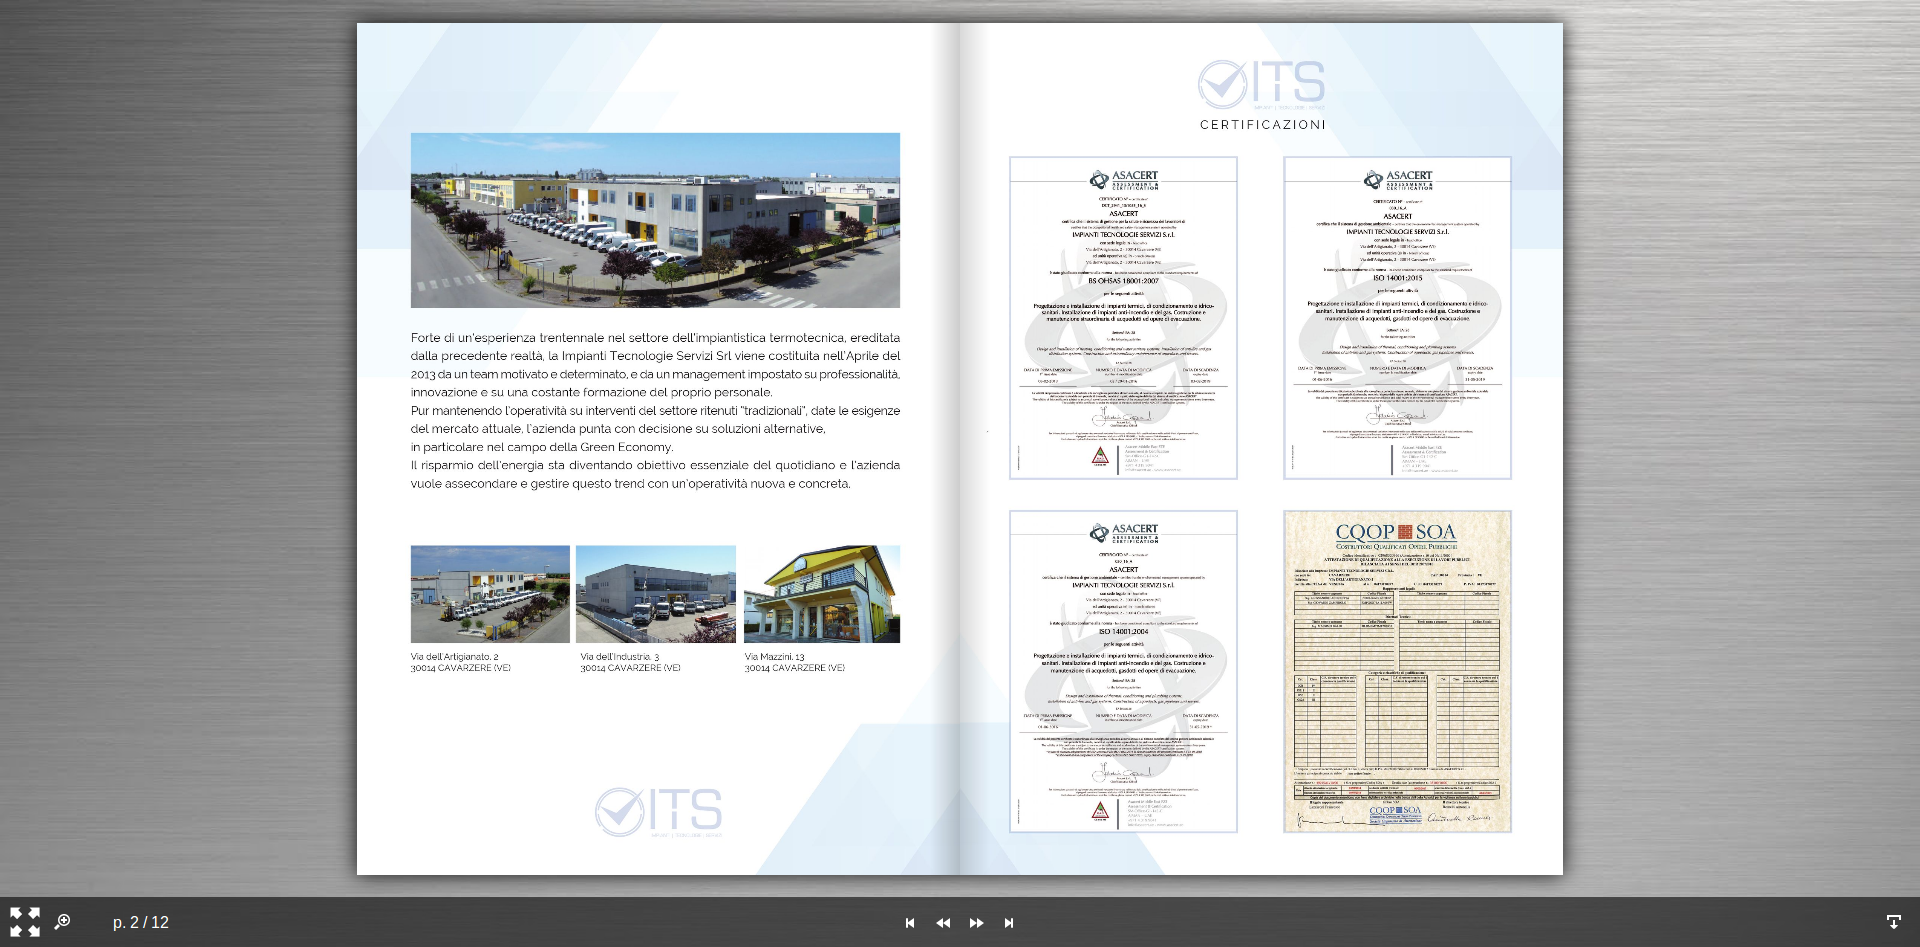
\includegraphics[width=1\textwidth]{img/Catalogo}
\caption{Catalogo - \url{http://www.youblisher.com/p/1700651-n-Touch/} \label{Catalogo}}
\end{figure}


\paragraph{What - Cosa offre il sito?}
La maggior parte della Home Page è impiegata per rispondere a questa domanda. Purtroppo, come già accennato, la prima vista non offre nessun informazione adeguata e il logo non aiuta a migliorare la situazione.
Le successive presentazioni dei servizi e prodotti permettono di identificare un possibile target di clientela, anche se la mancanza di informazioni relative ai prezzo non permette di effettuare un paragone con le esigenze dell'utente.\\
Trovo infelice la scelta di presentare i cataloghi visibili in figura \ref{"Home Page - Scroll 2"} come delle vere e proprie riviste cartacee (figura \ref{Catalogo}): le modalità di lettura sono ovviamente diverse tra web e supporto cartaceo e, tale scelta, oltre ad essere pesante da caricare, affatica la lettura e il reperimento delle informazioni necessarie.

\paragraph{When - Quali sono le ultime novità?}
Niente offre una risposta a questa domanda. Certo, i prodotti esposti e il design usato sembra moderno e recente, ma non c'è nulla che dia un idea concreta. Anzi, in basso a destra, nel footer in figura \ref{"Home Page - Scroll 8"}, viene riportata come anno di copyright il 2016. Ciò da un senso di abbandono del sito da parte dei gestori e fa sorgere dubbi sull'affidabilità e l'attuale validità dei contenuti.
 
\paragraph{How - Come faccio ad ottenere ciò che voglio?}
Il menu e la barra di ricerca attivabile cliccando sulla lente di ingrandimento permettono di navigare sul sito per ottenere le informazioni che si desiderano. Come anticipato nella sezione \ref{struttura}, la struttura interna non è bene organizzata, con la presenza di numerose pagine non raggiungibili in altra maniera se non effettuando svariati click all'interno delle nuove pagine. Una ristrutturazione del menu porterebbe grandi vantaggi a questo asse, permettendo una navigazione più diretta e veloce. \\ \\ In figura \ref{"Home Page - Scroll 8"} si può vedere come sia reso disponibile un form di contatto, l'email e il numero di telefono dell'azienda qualora si desiderasse contattarli. Tali informazioni sono ripetute in modo uguale nella sezione contatti, perdendo l'occasione di fornire qualche informazione aggiuntiva.

\IMG{Ricerca}
\subsubsection{Altre Considerazioni}
\begin{itemize}
	\item L'utente generalmente si aspetta che accada qualcosa quando si clicca su un immagine. In questa Home Page è vero solo per una parte delle immagini presenti. Sorprende che le immagini dei prodotti non siano cliccabili e ciò rischia di generare frustrazione all'utente; 
	\item Vi è la presenza di una metafora visiva non rispettata: la grande immagine che appare appena si entra nella Home Page, oltre a non essere cliccabile, riporta un finto bottone con la scritta "INNOVAZIONE". Data la sua forma, l'istinto è quello di cliccarlo, senza successo;
	\item La Home Page è decisamente troppo lunga e dispersiva. 8 scroll sono tanti e difficilmente gli utenti avranno la pazienza di farli tutti.;
	\item Le parole contenenti link cliccabili non vengono differenziate in alcun modo dal resto del testo, generando confusione all'utente che potrebbe non comprendere come poter ottenere le informazioni che desidera;
	\item La barra di ricerca in figura \ref{Ricerca} è attivabile cliccando la lente di ingrandimento a destra del menu e permette di scrivere molte parole. Lo svantaggio è il non rispettare le convenzioni sulla barra di ricerca a cui gli utenti sono abituati: una casella di testo e un pulsante con scritto "Cerca". Potrebbe essere una soluzione non gradita, anche perchè è necessario chiudere la funzionalità cliccando su una X se si desidera interrompere l'azione.
\end{itemize}
